\chapter{Models for  Search-Encounter Data}
\markboth{Search-Encounter}{}
\label{chapt.searchencounter}

\vspace{0.3cm}



The focus of this chapter should be these search-encounter models.
What do we mean by this? Probably better to say ``models for
search-encounter data''. These are models that arise where you get
actual location data of individuals not biased by trap locations but
rather by searching space in some fashion. In most cases both
detection probability and movement parameters are resolvable. i.e.,
models that preserve the these movement outcomes -- the $u_{it}$ variables.
The models we differentiate here depend on a number of
things related to data structure or protocol -- basically whether or
not we record the exact location and how we record it. All models have
an underlying movement model which may be completely latent or not.

How exactly
are these different from models for data from fixed arrays?  (1)
sample units are either continuous space polygons or lines, not
points; (2) we have location information that is not biased by trap
locations (but is biased by the observation device somehow); (3)
because we have direct observations of location that exist independent
of traps we can often build an explicit model of space usage or an
explicit movement model.

A few variations of the models exist -- a long sample path through a
sample region where we note the locations of individuals seen along
the way, {\it and their identity} (this is different from distance
sampling int hat sense). Or we could search a region systematically
and so forth.  
The canonical situation is Royle and Young (2008) which involved a
plot search for lizards. They assumed the plot was uniformly searched
which justified the assumption of constant $p$ within the plot
boundaries. The data set was $\ge 1$ location observations for each of
a sample of $n$ individuals. 
The recent paper by Efford XXXX
discussed likelihood analysis of similar models. In the jargon of
\mbox{\tt secr} such models are referred to as models for {\it polygon detectors}.
 An extension of this model was described
by \citep{royle_etal:2011mee}.  

Search-encounter models also provide something of a bridge between the
standard models for fixed trap arrays (e.g., Chapt. \ref{chapt.scr0}),
and the models of \citep{chandler_royle:2012} where no individual
identity is present. The latter are search-encounter models where the
movement process (and outcomes) are completely latent. Another type of
model is SCR/DS -- this is a SCR model with ..................

\section{Search-Encounter sampling designs}

For our purposes here we recognize 4 basic sampling designs, each of
which might come with more than 1 distinct sampling protocols. In
later sections of this chapter we will do some examples but not of all
of them. 

{\flushleft \bf Design 1: Fixed Search Path.}  The ideal situation is
where we have a continuous search-path or lines, or multiple such
lines, in some region (Fig. XXXX 1 XXXXX). This is the type of problem described
by Royle et al. (2011 MEE). We assume the path or lines are laid out a
priori in some manner that is done independent of the activity centers
of individuals and the collection of data does not affect the
lines. Sometimes the lines are within well-defined polygons but the
polygon boundaries are not meaningful in terms of the observation
process.  A number of variations of the data collection protocol are
possible:
\begin{itemize}
 \item[] Protocol (1a) has us just record the locations of individuals
 \item[] Protocol (1b) has us record location of individuals AND
   location on the transect where we observed the individual
 \item[] Protocol (1c) has us record neither of those things, instead
   we record the closest perpendicular distance. This is a typical
   distance sampling situation which produces exactly a DS type of a
   model (or a CR-DS model). We don't recommend recording closest
   perpendicular distance and we don't discuss these models too much
   here
 \item[] Protocol (1d) . In this case, observations are restricted to
   the line itself. We imagine that the line is evolving in response
   to search activity. It is not quite like the other ones so let's
   call it ``ad hoc''. In this case we use small bins as traps and the
   length of the line in each grid as a covariate. Unstructured survey
   data. Thompson et al. and Russell et al.
 \end{itemize}


{\flushleft \bf Design 2: Uniform search intensity.}
In this case we have one or more  well-defined sample areas (polygons), such as a quadrat or
a transect, and we imagine that the area is uniformly searched so that
$p = p_0$ is constant within the search area.  Sampling produces
locations of individuals within the well-defined boundaries of the
sample area. The polygon boundaries defining the sample unit are  important because it tells us that $p=0$ by design outside of the boundary.

Using the example from the Figure above, we could imagine that each
quadrat was uniformly searched. The individual quadrat boundaries are
irrelevant and we only need to be concerned about the ``total''
boundary of the composite polygon (the intersection of all little
ones). That said for analysis in BUGS it is easier to work with square
polygons.  We show a simulation example here and we analyze it either
using a bivariate normal movement model or else a 2-d random walk type
of model.  But we don't provide a real example as Royle and Dorazio
2008 did a reanalysis of the lizard data and see also Efford (XXXX).


{\flushleft \bf Design 3: bad implementation of 1 or 2}
(3)	Design 3 is based on a bad implementation of Design 1 or 2. We set up search polygons (e.g., the grid cells of above figure) and record locations of encountered individuals but we do not do a uniform search of quadrats and we forgot to record the GPS path. 
 Analysis of this design: We imagine that we can assume a uniform search intensity here and maybe it won't be so bad.  We should do a simulation study of this somehow. I am working on methods to lay down some standard sets of lines for simulating data, and then ignoring the lines in doing an analysis.
Alternative 2 for analysis: We could map each location to the CENTER of the grid cell and pretend this is trap array (traps at center of each grid). This was the idea of Kery et al. and some other papers.

{\flushleft \bf Design 4: Really bad implementation of 1 or 2}
(4)	Design 4: In this case we screw up even further and forget to record the locations of individuals within a bunch of quadrats.  I believe Richard has been thinking along these lines - using the underlying movement model as a latent model.
a.	Protocol (4a) - we imagine that you could have counts BY individual identity within each quadrat. Not sure what analysis model this would be
b.	Protocol (4b) - we DON'T have individual identities but just total counts. This is Chandler and Royle (2012/13).

For the book chapter I think my plan is to lay out these various data types or designs (a typology of models I guess), provide some simulation code, and a few limited analyses (not of every type) either of simulated data or real examples. Perhaps the MHB example from the MEE paper and the lizard data from Royle and Young and possibly the Fisher data from Thompson et al. or lion data from Robin Russell. That is too much material.

Example 1:  Analysis of the Swiss MHB survey using Design 1
Example 1b: Lizard data. No need to analyze this as it was done in RD book. Mention polygon detectors in secr.
Example 2: Fisher data possibly - lion data or -- or  Capricaillie data?


\section{Inference for Search-Encounter Designs}

We cover the basic Design 1 here which also is relevant to Design 2 as a special case.

Analysis of protocols 1a is that of Royle et al. (2011).  
The model:  

just copy out of Royle et al....

#u[I,t]  ~ bvn( s[i], sigma^2)
#Log(h(u[I,t],x)) = beta0 + beta1*dist(u[I,t],x)
#Total hazard is this:
#H(u[I,t]) = exp(beta0)* sum_{j} exp(beta1*dist(u[I,t],x[j])
#x[j] = point on line
#Then: p[I,t] = 1-exp(-H(u[I,t]))

\subsection{Example}
1.2. Example: Simulator and WinBUGS code for this example [in repo]

\begin{verbatim}
> wbout
Inference for Bugs model at "model0.txt", fit using jags,
 3 chains, each with 5000 iterations (first 1000 discarded)
 n.sims = 12000 iterations saved
         mu.vect sd.vect    2.5%     25%     50%     75%   97.5%  Rhat n.eff
N         94.448   5.237  81.000  92.000  96.000  98.000 100.000 1.006   520
beta0     -0.539   0.743  -1.714  -1.072  -0.637  -0.102   1.258 1.042    54
beta1    -11.943   2.196 -17.229 -13.236 -11.665 -10.375  -8.378 1.035    62
psi        0.936   0.056   0.792   0.908   0.951   0.979   0.998 1.005   650
sigma      0.340   0.043   0.268   0.309   0.337   0.366   0.436 1.004   820
deviance 206.987  25.474 160.405 189.069 205.779 224.080 259.491 1.017   130

For each parameter, n.eff is a crude measure of effective sample size,
and Rhat is the potential scale reduction factor (at convergence, Rhat=1).

DIC info (using the rule, pD = var(deviance)/2)
pD = 319.4 and DIC = 526.3
DIC is an estimate of expected predictive error (lower deviance is better).
\end{verbatim}







\subsection{Hard plot boundaries}
1.3. Hard quadrat boundaries: Quadrat boundaries might be relevant or might not be.  If they are then, for Bayesian analysis, a value of u outside the boundary has p forced to 0, its as simple as that. 
In general, we define p[I,t] = p[I,t]*I(u in X).
We see how this relates to the uniform search intensity model.  P[I,t] = p0 then defines precisely the model of Royle and Young (2008). 

\subsection{Analysis of other protocols}

Analysis of 1b is a distance-sampling like model but with an additional hierarchical structure the describes the individual location scatter about the home range center. This is precisely a type of DS with measurement error. Analysis of 1c is a similar idea except it represents an explicit model misspecification since one is approximating the observation process by the nearest perpendicular to the line.  Analysis of 1d is the ``unstructured survey data'' like from Thompson et al. or Russell et al.  Note also that the capcrap paper is a version of this - grids or polygons were sampled but no information on the search path is available. This could be a Design 3 problem but that is excess computation I think. 
Protocol (1b) has us record location of individuals AND location on the transect where we observed the individual. This is an easier problem I think, but you have to account for ``not seen'' prior  to x0 so maybe some kind of a cumulative hazard model or something. 
Protocol (1c) has us record neither of those things, instead we record the closest perpendicular distance. This is a typical distance sampling situation which produces exactly a DS type of a model (or a CR-DS model). We don't recommend recording closest perpendicular distance and we don't discuss these models too much here
Protocol (1d) . In this case, observations are restricted to the line itself. We imagine that the line is evolving in response to search activity. It is not quite like the other ones so let's call it ``ad hoc''. In this case we use small bins as traps and the length of the line in each grid as a covariate. Thompson et al. and Russell et al.
Simulation results -----------------




Section: Design 3: Ad hoc implementation of Design 1.
We don't do anything new in terms of modeling here but we look at how bad do we do if we don't have the search path and use the USI model?  We consider 4 cases: Case 1 and 2: regular searching of low and high intensity. E.g., for a 1 unit block, then we can have a sinusoid track through each block of length 1.5 or 2 and then 4 or 5 km.   For case 3 and 4 we use heterogeneity in search intensity.

Section: Design 4 -- no location info

1.	Imagine we have a bunch of quadrats or segments that are contiguous and we do the surveys like above and record counts PER individual  but no other sampling information.
2.	Design 4b: We don't record individual ID.
Basic concept is that correlation among quadrats is induced. Like Chandler and Royle..... This ties us to that paper.




\section{Capricaillie crap}

\begin{comment}
We provide an example of the Poisson model from
 \citet{mollet_etal:2012}, who obtained a population
size estimate  of a large forest grouse species known as the
capracaillie in a region of Switzerland.

In this study,
8 forest stands  that represent all available habitat of the
species were sampled. Each of the stands was divided into a number of
fragments, each of
sufficient size to sample in a meaningful way, creating 39 patches of around
30-70 ha each. For modeling we further divided each patch roughly in half to
create 78 spatial sample units -- so scat samples could be associated to one of
the 78 sub-units. This was done mostly for the purpose of creating spatial
replicates. If the 39 larger units were used there were relatively little
realized spatial replicates.
We did not use finer scale things because searching was rather opportunistic
and haphazard within a unit. Observers searched out what they thought was
good opportunity to find scats but we don't know the whole extnet of
sampling..........

Importantly, the sample units are actually large forest
patches on the order of tens of ha each, but variable in size. Data
were {\it not} collected by coordinates of observations but rather
just recorded to the specific patch in which the observation was
encountered. To accomodate this we defined ${\bf s}_{i}$ to be a
discrete
random variable taking on values...........................

Forest patches were searched for scat which was
situation in which discrete patches of habitat are searched using some
method and it might be convenient (or occur inadvertently) to
associate samples to the patch level instead of recording observation
locations. In this case we might use a model $s[i] \sim dcat(probs[])$
where $probs[]$ are the probabilities that an individual inhabits a
particular patch.

samples are spatial encounter frequencies of scat essentially and so
it makes sense to think of them as Poisson or other.
In fact there's a bit of opportunistic thinning going on but we'll view
this as random thinning and still asert that the encounter frequencies
are Poisson with constant $\lambda_{0}$ and individual intensity that
depends on distance according to the bivariate normal model.



\begin{figure}
\centering
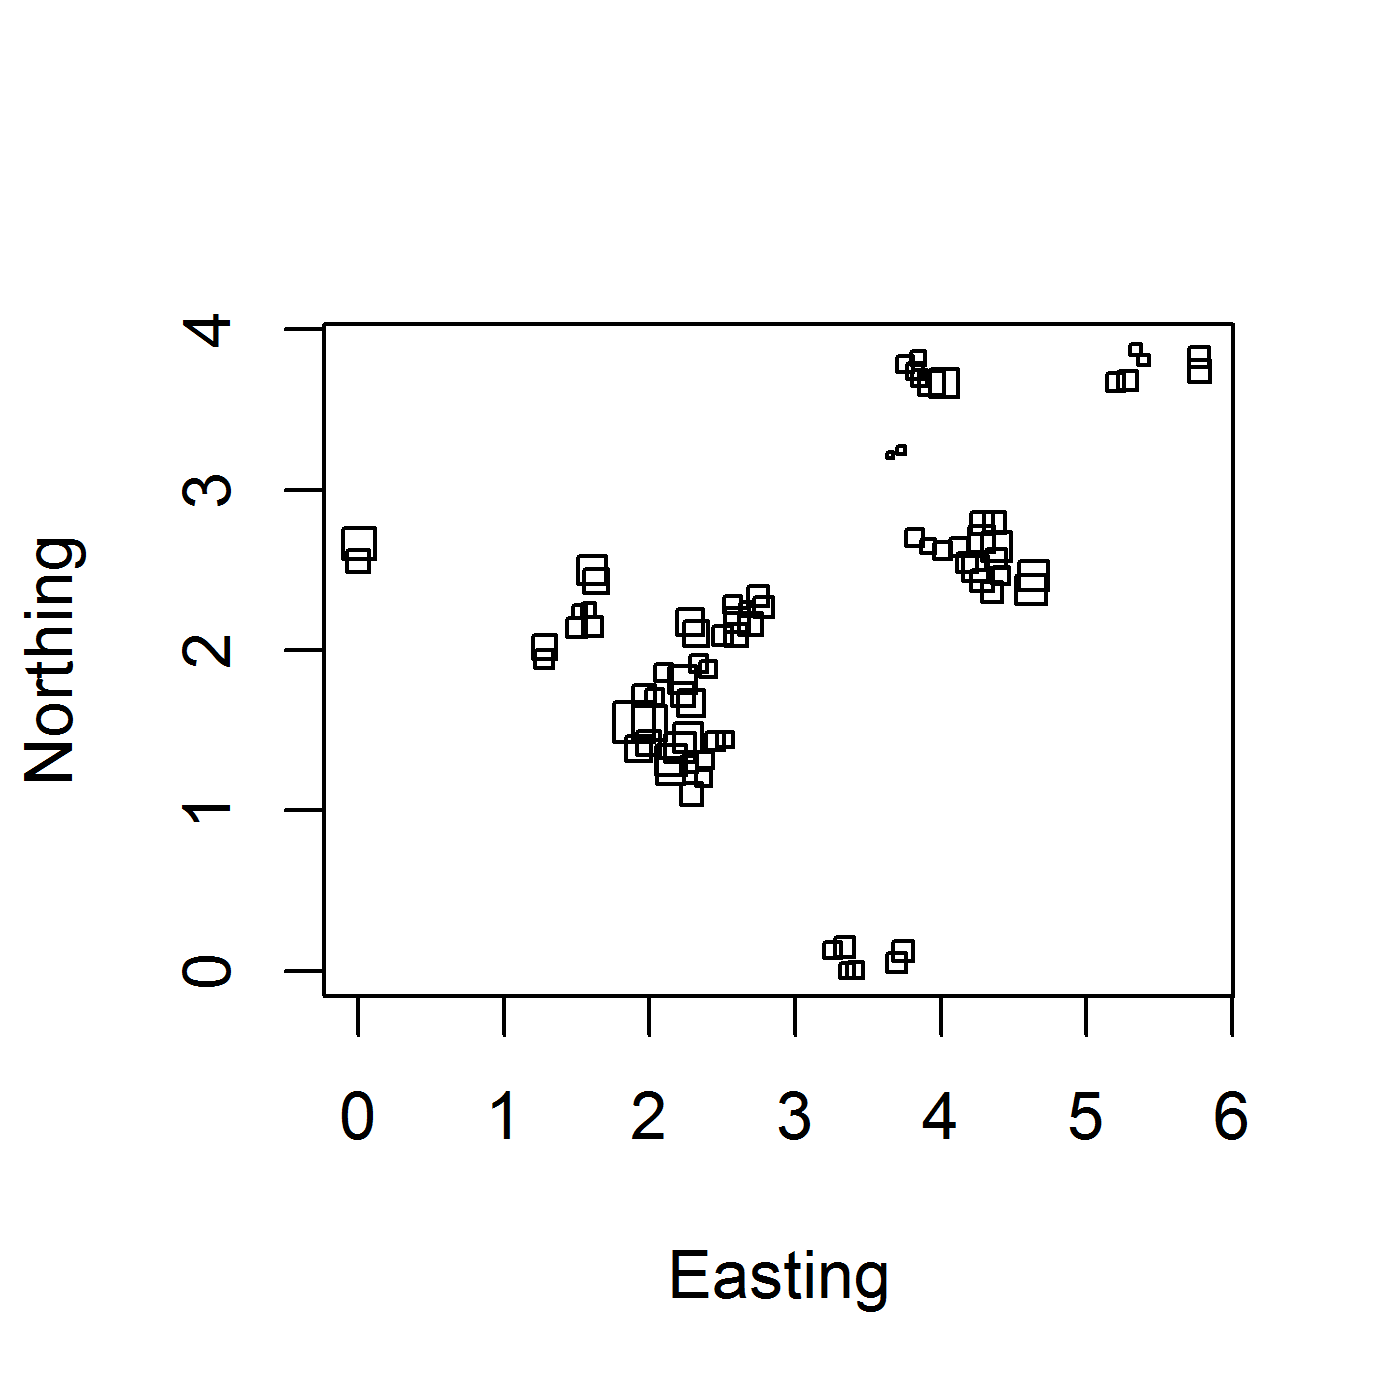
\includegraphics[width=3.5in,height=3.5in]{Ch5/figs/Cap-fragments.png}
\label{poisson-mn.fig.capfrags}
\caption{Relative size and position of 78 forest fragments sampled for
  capricaillie crap.}
\end{figure}


Each of the 44 units
could be sampled by one person in
one day's work (6-8 hours). Within each unit, we focused our search
for droppings on the areas below roosting trees and feeding trees,
respectively, in hiding sites, along internal forest edges, around
root plates and on tree stumps (cf. Jacob et al. 2010). These habitat
elements are the ones preferred by the birds in winter at a small
spatial scale (Bollmann et al. 2005; Mollet unpublished data).
Five spatial units ($I_a$, $S_a$, $S_b$, $H_a$, $T_a$, Table 2) could
not be sampled because of time constraints (too few days with
favorable weather conditions), resulting in 39 units sampled. For the
same reason, three units $(I_b, W_1, W_a)$ were sampled only
once. Access to the area B (Fig. 2) is possible only in late
spring. In 2009, sampling started on 20 April, and the three units in
area B could be sampled only once (rapid snow melting towards the end
of April precluded repetition of sampling here). All other units were
sampled twice.




\subsection{model}

activity centers were uniformly distributed to each of the 78
fragments in proportion to area of the forest patch within which each
fragment was located.


We parameterized activity centers by a discrete state-space with elements
corresponding to the 8 larger fragments. Moreover, home ranges were allocated
to each fragment in  proportion to area. i.e., we assume
define $\lambda_{frag} = A_{frag} \lambda_{0}$, and then:
\[
 N_{frag} \sim Poisson( A_{frag} \lambda_{0} )
\]
This assumption implies the following prior distribution on ${\bf s}_{i}$ (Chapt.
XYZ; Converse and Royle 2012):
\[
{\bf s}_{i} \sim  \mbox{Categorical}(  \pi_{frag} )
\]
with
\[
 \pi_{frag} = \frac{ \lambda_{frag} }{\sum_{frag} \lambda_{frag}}
\]


Observation model:

Each of the 78 fragments is its own sample unit which we index to the
center point of the fragment. No finer scale information is made about
the observation locations.
Let $y_{ij}$ be  the number of times individual $i$ encountered in stand $j$.
Note these are not unique droppings but rather unique clusters of
droppings because a grouse roosting in a tree might leave a number of
droppings and only one of them was sampled\footnote{perhaps this is
  too optimistic of an assessment?}.

\end{comment}





